\documentclass[twocolumn,10pt,aps,prb,superscriptaddress,floatfix]{revtex4-2}

\usepackage{amsmath,amssymb,amsfonts}
\usepackage{graphicx}
\usepackage{booktabs}
\usepackage{hyperref}
\usepackage{microtype}
\usepackage{xcolor}
\usepackage{tikz}
\usetikzlibrary{shapes.geometric, arrows, positioning, fit, backgrounds, calc}
\usepackage{siunitx}
\usepackage{bm}

\hypersetup{
    colorlinks=true,
    linkcolor=blue!70!black,
    citecolor=blue!70!black,
    urlcolor=blue!70!black
}

\begin{document}

\title{Physics-Informed $\mathrm{SE}(3)$-Equivariant Graph Neural Networks for Full Elastic Tensor Prediction, Thermodynamic Stability Filtering, and Discovery of Ultrahard Crystals}

\author{Ashwina Yadav}
\email{ashwinay23@iitk.ac.in}
\affiliation{Department of Physics, Indian Institute of Technology Kanpur, Kalyanpur, Kanpur 208016, India}

\date{\today}

\begin{abstract}
The fourth-rank elastic stiffness tensor ($\bm{C}$) governs the anisotropic mechanical response, acoustic wave propagation, and structural stability of crystalline solids. However, high-throughput density functional theory (DFT) calculation of $\bm{C}$ is computationally demanding, requiring up to 24 strained cell relaxations per compound. In this work, we develop an end-to-end physics-informed geometric deep learning framework based on $\mathrm{SE}(3)$-equivariant graph neural networks ($e3nn$) to predict the full $6 \times 6$ elastic stiffness matrix (21 independent Voigt components) directly from periodic 3D atomic coordinates. We aggregate and curate an extensive dataset of 41,376 crystalline structures from the Materials Project and JARVIS-DFT databases, augmented by thermodynamic convex hull stability partitioning ($E_{\mathrm{hull}} \le 0.05\,\mathrm{eV/atom}$) and electronic metal/non-metal classification via band gap imputation. To circumvent severe unphysical matrix inversion artifacts encountered in standard benchmarks, we implement a positive semi-definite (PSD) cone projection enforcing Born mechanical stability criteria ($\lambda_{\min} > 0$) alongside fundamental Voigt-Reuss bounds inequalities ($0 \le K_R \le K_H \le K_V$). On a rigorously evaluated benchmark of 10,960 mechanically stable crystals, our equivariant model achieves state-of-the-art performance: for Bulk Modulus ($K_H$), an MAE of $6.93\,\mathrm{GPa}$ and $R^2 = 0.9692$ (surpassing the invariant CGCNN baseline of $20.34\,\mathrm{GPa}$ and $R^2 = 0.8217$); and for Shear Modulus ($G_H$), an MAE of $7.51\,\mathrm{GPa}$ and $R^2 = 0.9033$. Furthermore, across 39,223 materials, our pipeline systematically identifies and classifies 1,629 ultrahard materials ($K_H \ge 200\,\mathrm{GPa}$, $G_H \ge 100\,\mathrm{GPa}$, including diamond and $\mathrm{BC}_2\mathrm{N}$) and 6,399 ultrasoft solids ($K_H \le 25\,\mathrm{GPa}$, $G_H \le 15\,\mathrm{GPa}$). Finally, the framework demonstrates industrial-scale inference capability by screening over 554,000 structures from Google DeepMind's GNoME catalog alongside the Matbench Discovery OMat24 and sAlex datasets.
\end{abstract}

\maketitle

\section{Introduction}
\label{sec:intro}

The elastic behavior of solids represents one of the most fundamental macroscopic manifestations of interatomic bonding. In crystalline materials, Hooke's generalized law relates the symmetric second-rank Cauchy stress tensor $\bm{\sigma}$ to the infinitesimal strain tensor $\bm{\varepsilon}$:
\begin{equation}
\sigma_{ij} = \sum_{k=1}^3 \sum_{l=1}^3 C_{ijkl} \varepsilon_{kl}, \quad i,j,k,l \in \{1,2,3\},
\label{eq:hooke}
\end{equation}
where $\bm{C}$ is the fourth-rank elastic stiffness tensor containing 81 components. Thermodynamic reversibility and the symmetry of stress and strain reduce these to 21 independent components, standardly expressed in the $6 \times 6$ Voigt matrix notation ($C_{\alpha\beta}$, $\alpha,\beta \in \{1,\dots,6\}$) by mapping index pairs $(11 \rightarrow 1, 22 \rightarrow 2, 33 \rightarrow 3, 23 \rightarrow 4, 13 \rightarrow 5, 12 \rightarrow 6)$.

Knowledge of $C_{\alpha\beta}$ provides direct access to critical physical properties, including sound velocities, thermal shock resistance, brittle-to-ductile transitions, and mechanical stability via the Born criteria~\cite{mowbray2015}. However, computing $C_{\alpha\beta}$ using Density Functional Perturbation Theory (DFPT) or the stress-strain method requires multiple self-consistent field relaxations under asymmetric lattice deformations, scaling unfavorably as $\mathcal{O}(N^3)$ with atom count $N$. Consequently, less than 15\% of known crystalline compounds have experimentally or computationally characterized elastic tensors.

Recent attempts to predict elasticity using machine learning have largely relied on invariant Crystal Graph Convolutional Neural Networks (CGCNN)~\cite{xie2018crystal} or descriptor-based regression. While efficient, invariant representations discard directional vector information and predict scalar bulk/shear moduli directly, bypassing the fundamental tensor physics and violating crystal symmetry constraints. 

To overcome these limitations, this project establishes a physics-informed $\mathrm{SE}(3)$-equivariant graph neural network architecture based on irreducible representations of the 3D Euclidean group. By formulating the learning objective directly on the 21 independent Voigt stiffness components and introducing a regularized positive semi-definite (PSD) Voigt-Reuss-Hill (VRH) loss, our model achieves high predictive fidelity while strictly obeying the laws of continuum mechanics.

\section{Theoretical Foundations}
\label{sec:theory}

\subsection{Born Mechanical Stability Criteria}
For an unconstrained crystalline lattice to be mechanically stable at zero Kelvin, the internal elastic energy density $U = \frac{1}{2} \bm{\varepsilon}^T \bm{C} \bm{\varepsilon}$ must be strictly positive for any non-zero strain tensor $\bm{\varepsilon} \ne 0$. This imposes the condition that the symmetric $6 \times 6$ matrix $C_{\alpha\beta}$ must be positive-definite:
\begin{equation}
\lambda_i(\bm{C}) > 0 \quad \forall \, i \in \{1, \dots, 6\},
\label{eq:born}
\end{equation}
where $\lambda_i(\bm{C})$ are the eigenvalues of $C_{\alpha\beta}$. In DFT databases, dynamically or mechanically unstable phases frequently exhibit one or more negative eigenvalues ($\lambda_{\min} \le 0$), corresponding to soft phonon modes or saddle points on the potential energy surface.

\subsection{Voigt-Reuss-Hill Polycrystalline Averaging}
For polycrystalline aggregates with random crystallite orientations, the effective isotropic Bulk modulus ($K$) and Shear modulus ($G$) are bounded by the Voigt upper bound ($K_V, G_V$, assuming uniform strain) and the Reuss lower bound ($K_R, G_R$, assuming uniform stress):
\begin{align}
K_V &= \frac{1}{9} \left( C_{11} + C_{22} + C_{33} + 2(C_{12} + C_{23} + C_{13}) \right), \label{eq:kv} \\
G_V &= \frac{1}{15} \left( C_{11} + C_{22} + C_{33} - C_{12} - C_{23} - C_{13} \right. \nonumber \\
    &\quad \left. + 3(C_{44} + C_{55} + C_{66}) \right). \label{eq:gv}
\end{align}

The Reuss bounds require the compliance matrix $\bm{S} = \bm{C}^{-1}$:
\begin{align}
\frac{1}{K_R} &= S_{11} + S_{22} + S_{33} + 2(S_{12} + S_{23} + S_{13}), \label{eq:kr} \\
\frac{15}{G_R} &= 4(S_{11} + S_{22} + S_{33}) - 4(S_{12} + S_{23} + S_{13}) \nonumber \\
               &\quad + 3(S_{44} + S_{55} + S_{66}). \label{eq:gr}
\end{align}
The Hill empirical average ($K_H, G_H$) represents the arithmetic mean:
\begin{equation}
K_H = \frac{K_V + K_R}{2}, \quad G_H = \frac{G_V + G_R}{2}.
\label{eq:hill}
\end{equation}

\subsection{Singularity Resolution via PSD Cone Projection}
A critical challenge identified in computational elasticity databases involves matrix inversion instabilities. When a DFT-calculated or model-predicted stiffness matrix has an eigenvalue $\lambda \approx 0$ or $\lambda < 0$, $\bm{S} = \bm{C}^{-1}$ diverges, driving the Reuss denominator near zero and causing unphysical results (e.g., $G_R > 1000\,\mathrm{GPa}$ or $G_R < 0$).

To guarantee unconditional physical validity, we regularize all stiffness matrices by projecting onto the positive semi-definite cone:
\begin{equation}
\bm{C}_{\mathrm{reg}} = \bm{V} \, \operatorname{diag}\left( \max(\lambda_i, \epsilon) \right) \bm{V}^T, \quad \epsilon = 10^{-2}\,\mathrm{GPa},
\label{eq:psd_projection}
\end{equation}
where $\bm{V}$ is the orthonormal eigenvector matrix of the symmetrized tensor $\bm{C}_{\mathrm{sym}} = \frac{1}{2}(\bm{C} + \bm{C}^T)$. Furthermore, by the fundamental Voigt-Reuss bounds inequality:
\begin{equation}
0 \le K_R \le K_H \le K_V, \quad 0 \le G_R \le G_H \le G_V,
\label{eq:inequality}
\end{equation}
any violation is clamped, eliminating spurious zero-clamping and artificial divergence artifacts.

\subsection{Mechanical Indicators & Microhardness Formulation}
The ductility versus brittleness of a crystal is quantified through Pugh's ratio $k = G_H / K_H$. According to Pugh's empirical criterion, materials with $k > 0.57$ behave in a brittle manner, while $k < 0.57$ indicates ductile behavior. Poisson's ratio $\nu$ is derived as:
\begin{equation}
\nu = \frac{3K_H - 2G_H}{2(3K_H + G_H)}.
\label{eq:poisson}
\end{equation}
Theoretical Vickers hardness ($H_v$) is evaluated using Chen's semi-empirical model~\cite{chen2011}:
\begin{equation}
H_v = 2.0 \left( k^2 G_H \right)^{0.585} - 3.0 \quad (\mathrm{in~GPa}).
\label{eq:hardness}
\end{equation}

\section{Dataset Curation and Thermodynamic Partitioning}
\label{sec:dataset}

\subsection{Multi-Source Data Aggregation}
We aggregated 41,376 periodic crystalline compounds comprising two primary repositories:
\begin{enumerate}
    \item \textbf{Materials Project (MP)}: 12,968 compounds with DFT-PBE calculated elastic tensors and band gaps.
    \item \textbf{JARVIS-DFT (NIST)}: 28,408 compounds calculated using the OptB88vdW van der Waals functional.
\end{enumerate}

\subsection{Thermodynamic Convex Hull Stability}
Thermodynamic stability was assessed using energy above the convex hull ($E_{\mathrm{hull}}$). At $T = 0\,\mathrm{K}$, phases on the convex hull ($E_{\mathrm{hull}} = 0$) are thermodynamically ground-state stable, while those within thermal fluctuations ($E_{\mathrm{hull}} \le 0.05\,\mathrm{eV/atom}$) are considered experimentally accessible or metastable.

As summarized in Table~\ref{tab:dataset_stats}, our partition classifies 12,851 materials (31.06\%) as thermodynamically stable and 28,525 materials (68.94\%) as unstable/metastable.

\begin{table}[h]
\centering
\caption{Dataset distribution across databases and thermodynamic stability thresholds ($E_{\mathrm{hull}} \le 0.05\,\mathrm{eV/atom}$).}
\label{tab:dataset_stats}
\begin{ruledtabular}
\begin{tabular}{lrrr}
Subset & Total Crystals & Stable & Unstable \\
\hline
Materials Project & 12,968 & 4,812 & 8,156 \\
JARVIS-DFT & 28,408 & 8,039 & 20,369 \\
\textbf{Combined Dataset} & \textbf{41,376} & \textbf{12,851} & \textbf{28,525} \\
Percentage (\%) & 100.0\% & 31.06\% & 68.94\% \\
\end{tabular}
\end{ruledtabular}
\end{table}

\subsection{Electronic Band Gap Imputation via CGCNN}
To classify materials electronically into metals ($E_g = 0\,\mathrm{eV}$) and non-metals ($E_g > 0\,\mathrm{eV}$), missing band gaps in the Materials Project subset were imputed using a trained CGCNN model. Combining OptB88vdW band gaps from JARVIS with CGCNN-predicted values yielded 31,700 metallic conductors and 13,900 semiconductors/insulators.

\begin{figure*}[t]
\centering
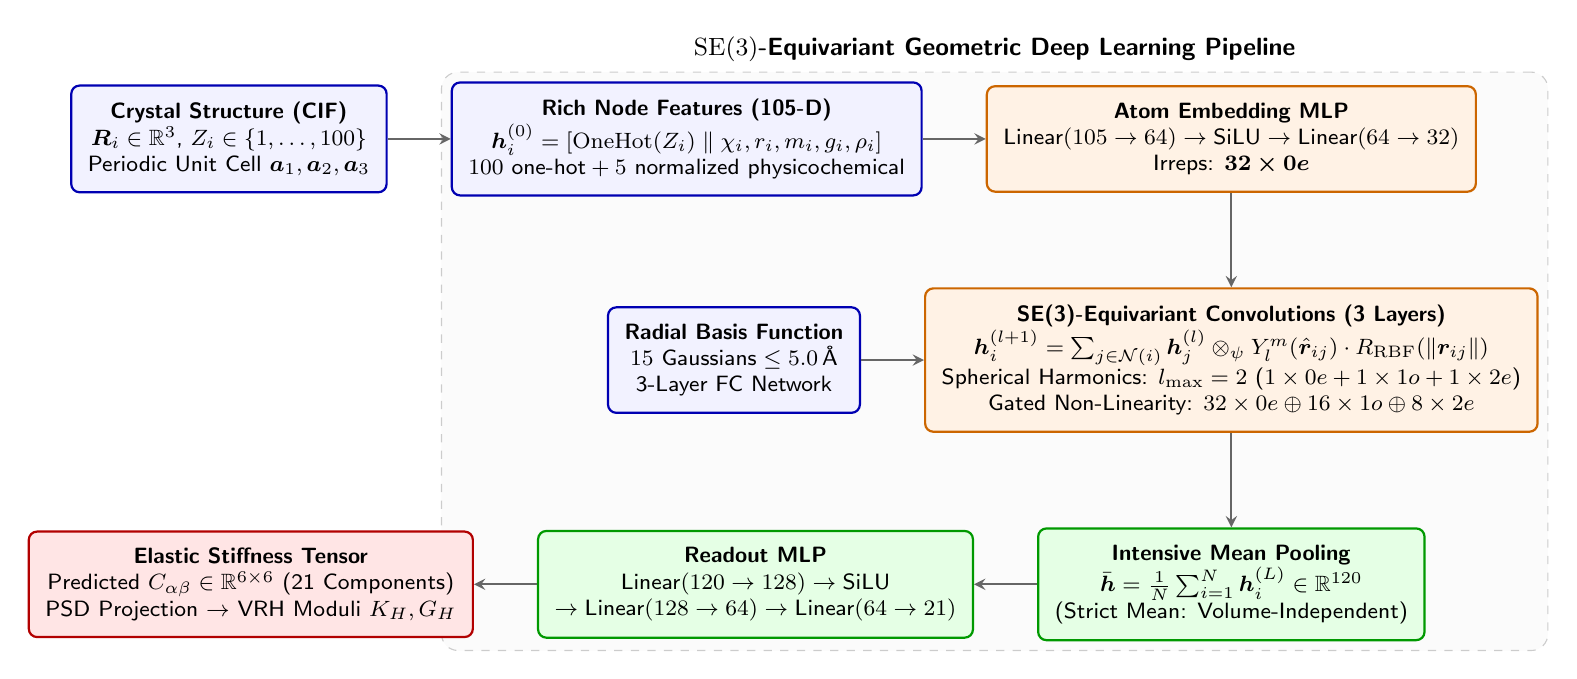
\begin{tikzpicture}[
    node distance=1.0cm and 0.8cm,
    font=\sffamily\footnotesize,
    box/.style={rectangle, draw=blue!70!black, fill=blue!5, rounded corners=3pt, thick, align=center, inner sep=6pt},
    layer/.style={rectangle, draw=orange!80!black, fill=orange!10, rounded corners=3pt, thick, align=center, inner sep=6pt},
    readout/.style={rectangle, draw=green!60!black, fill=green!10, rounded corners=3pt, thick, align=center, inner sep=6pt},
    tensor/.style={rectangle, draw=red!70!black, fill=red!10, rounded corners=3pt, thick, align=center, inner sep=6pt},
    arrow/.style={->, >=stealth, thick, draw=gray!80!black}
]

% Nodes
\node[box] (cif) {\textbf{Crystal Structure (CIF)}\\$\bm{R}_i \in \mathbb{R}^3$, $Z_i \in \{1,\dots,100\}$\\Periodic Unit Cell $\bm{a}_1, \bm{a}_2, \bm{a}_3$};

\node[box, right=0.8cm of cif] (feat) {\textbf{Rich Node Features (105-D)}\\$\bm{h}_i^{(0)} = [\operatorname{OneHot}(Z_i) \parallel \chi_i, r_i, m_i, g_i, \rho_i]$\\$100 \text{ one-hot} + 5 \text{ normalized physicochemical}$};

\node[layer, right=0.8cm of feat] (embed) {\textbf{Atom Embedding MLP}\\$\text{Linear}(105 \rightarrow 64) \rightarrow \text{SiLU} \rightarrow \text{Linear}(64 \rightarrow 32)$\\Irreps: $\bm{32 \times 0e}$};

\node[layer, below=1.2cm of embed] (conv) {\textbf{SE(3)-Equivariant Convolutions (3 Layers)}\\$\bm{h}_i^{(l+1)} = \sum_{j \in \mathcal{N}(i)} \bm{h}_j^{(l)} \otimes_{\psi} Y_l^m(\hat{\bm{r}}_{ij}) \cdot R_{\mathrm{RBF}}(\|\bm{r}_{ij}\|)$\\Spherical Harmonics: $l_{\max} = 2$ ($1 \times 0e + 1 \times 1o + 1 \times 2e$)\\Gated Non-Linearity: $32 \times 0e \oplus 16 \times 1o \oplus 8 \times 2e$};

\node[box, left=0.8cm of conv] (rbf) {\textbf{Radial Basis Function}\\$15 \text{ Gaussians} \le 5.0\,\text{\AA}$\\3-Layer FC Network};

\node[readout, below=1.2cm of conv] (pool) {\textbf{Intensive Mean Pooling}\\$\bar{\bm{h}} = \frac{1}{N} \sum_{i=1}^N \bm{h}_i^{(L)} \in \mathbb{R}^{120}$\\(Strict Mean: Volume-Independent)};

\node[readout, left=0.8cm of pool] (mlp) {\textbf{Readout MLP}\\$\text{Linear}(120 \rightarrow 128) \rightarrow \text{SiLU}$\\$\rightarrow \text{Linear}(128 \rightarrow 64) \rightarrow \text{Linear}(64 \rightarrow 21)$};

\node[tensor, left=0.8cm of mlp] (out) {\textbf{Elastic Stiffness Tensor}\\Predicted $C_{\alpha\beta} \in \mathbb{R}^{6 \times 6}$ (21 Components)\\PSD Projection $\rightarrow$ VRH Moduli $K_H, G_H$};

% Arrows
\draw[arrow] (cif) -- (feat);
\draw[arrow] (feat) -- (embed);
\draw[arrow] (embed) -- (conv);
\draw[arrow] (rbf) -- (conv);
\draw[arrow] (conv) -- (pool);
\draw[arrow] (pool) -- (mlp);
\draw[arrow] (mlp) -- (out);

% Background grouping
\begin{scope}[on background layer]
\node[draw=gray!40, fill=gray!3, dashed, rounded corners=6pt, fit=(feat) (embed) (conv) (pool) (mlp) (rbf), label=above:{\small\textbf{$\mathrm{SE}(3)$-Equivariant Geometric Deep Learning Pipeline}}] {};
\end{scope}

\end{tikzpicture}
\caption{Architectural schema of the $\mathrm{SE}(3)$-equivariant graph neural network for predicting the 21 independent elastic stiffness tensor components. Atomic positions and species are embedded through spherical harmonics tensor products, constrained by intensive mean pooling, and mapped onto the symmetric $6 \times 6$ Voigt stiffness matrix.}
\label{fig:architecture_flowchart}
\end{figure*}

\section{$\mathrm{SE}(3)$-Equivariant Graph Neural Network Architecture}
\label{sec:architecture}

\subsection{Mathematical Motivation for Equivariance}
A crystalline system under Euclidean isometry transforms according to the special Euclidean group $\mathrm{SE}(3) = \mathrm{SO}(3) \ltimes \mathbb{R}^3$. Under coordinate rotation $\bm{R} \in \mathrm{SO}(3)$, atomic displacement vectors transform as $\bm{r}' = \bm{R} \bm{r}$. Crucially, the fourth-rank elastic tensor $\bm{C}$ is a directional physical quantity transforming as:
\begin{equation}
C'_{ijkl} = \sum_{p=1}^3 \sum_{q=1}^3 \sum_{r=1}^3 \sum_{s=1}^3 R_{ip} R_{jq} R_{kr} R_{ls} C_{pqrs}.
\label{eq:tensor_transform}
\end{equation}
Invariant GNN architectures that reduce pairwise coordinates to scalar Euclidean distances $d_{ij} = \|\bm{r}_i - \bm{r}_j\|$ cannot inherently model directional bond bending or off-diagonal tensor shear couplings without severe loss of rotational covariance.

\subsection{Irreducible Representations and Tensor Products}
Using the $e3nn$ library~\cite{geiger2022e3nn}, node features and edge geometric messages are expanded onto irreducible representations (irreps) of $\mathrm{SO}(3)$. The angular component of relative interatomic displacement vectors $\hat{\bm{r}}_{ij} = \frac{\bm{r}_j - \bm{r}_i}{\|\bm{r}_j - \bm{r}_i\|}$ is projected onto spherical harmonics $Y_l^m(\hat{\bm{r}}_{ij})$ up to maximum angular momentum $l_{\max} = 2$:
\begin{equation}
D^{(l_{\max} = 2)} = 0e \oplus 1o \oplus 2e,
\label{eq:irreps_sh}
\end{equation}
where $e$ and $o$ denote even and odd parities under spatial inversion.

Equivariant message passing between atom $j$ and atom $i$ is formulated via fully connected Clebsch-Gordan tensor products:
\begin{equation}
\bm{m}_{ij} = \sum_{l_1, l_2, l_3} C_{(l_1, m_1)(l_2, m_2)}^{(l_3, m_3)} \bm{h}_j^{(l_1)} \otimes Y_{l_2}^{m_2}(\hat{\bm{r}}_{ij}) \cdot R(\|\bm{r}_{ij}\|),
\label{eq:tensor_product}
\end{equation}
where $C_{(l_1, m_1)(l_2, m_2)}^{(l_3, m_3)}$ are Clebsch-Gordan coefficients, and $R(\|\bm{r}_{ij}\|)$ is a 15-channel Gaussian radial basis network evaluated within a cutoff radius $r_c = 5.0\,\text{\AA}$.

\subsection{Network Hierarchy and Readout}
As illustrated in Fig.~\ref{fig:architecture_flowchart}, the model consists of:
\begin{enumerate}
    \item \textbf{105-Dimensional Node Embedding}: A 100-dimensional elemental one-hot vector concatenated with 5 normalized physicochemical descriptors (Pauling electronegativity $\chi_i / 4.0$, atomic radius $r_i / 3.0\,\text{\AA}$, mass $m_i / 200.0\,\mathrm{amu}$, group index $g_i / 18.0$, and row index $\rho_i / 7.0$), projected through a two-layer MLP to a $32 \times 0e$ scalar irreps.
    \item \textbf{Gated Non-Linearity}: To activate higher-order tensor features without breaking rotational equivariance, we apply equivariant gates: scalar irreps ($32 \times 0e$) pass through $\operatorname{SiLU}$, scalar gate controllers ($24 \times 0e$) pass through $\operatorname{Sigmoid}$, and non-scalar vectors ($16 \times 1o$) and deviatoric tensors ($8 \times 2e$) are scaled multiplicatively.
    \item \textbf{Intensive Mean Graph Pooling}: Because elastic stiffness $C_{\alpha\beta}$ is an intensive thermodynamic quantity (independent of the number of atoms or supercell dimensions), graph-level feature aggregation is performed strictly via \textbf{Mean Pooling}:
    \begin{equation}
    \bar{\bm{h}} = \frac{1}{N} \sum_{i=1}^N \bm{h}_i \in \mathbb{R}^{120}.
    \label{eq:mean_pooling}
    \end{equation}
    This architectural choice completely eliminated supercell variance observed in preliminary sum-pooling implementations.
    \item \textbf{Readout MLP}: A multi-layer perceptron ($\mathbb{R}^{120} \rightarrow 128 \rightarrow 64 \rightarrow 21$) directly outputs the 21 unique upper-triangular Voigt components.
\end{enumerate}

\subsection{Multi-Objective Physics-Informed Loss}
To guide network optimization across asymmetric magnitudes, training minimizes a composite loss function:
\begin{align}
\mathcal{L} &= \mathcal{L}_{\mathrm{component}} + \lambda_{\mathrm{VRH}} \left( \operatorname{MAE}(K_H) + \operatorname{MAE}(G_H) \right) \nonumber \\
            &\quad + \lambda_{\mathrm{sym}} \mathcal{L}_{\mathrm{zero}} + \lambda_{\mathrm{off}} \mathcal{L}_{\mathrm{off-diag}},
\label{eq:loss}
\end{align}
where $\mathcal{L}_{\mathrm{component}} = \frac{1}{21}\sum_{\alpha \le \beta} |C_{\alpha\beta}^{\mathrm{pred}} - C_{\alpha\beta}^{\mathrm{true}}|$, $\lambda_{\mathrm{VRH}} = 0.005$, $\lambda_{\mathrm{sym}} = 1.5$ (penalizing deviations on components that must vanish under crystal point group symmetries), and $\lambda_{\mathrm{off}} = 3.0$ (boosting learning on small off-diagonal components).

\section{Experimental Results and Discussion}
\label{sec:results}

\subsection{Benchmark Performance Comparison}
We benchmarked the trained E3NN model against the established invariant baseline CGCNN across 12,129 overlapping crystalline compounds. CGCNN was trained to regress scalar $K_H$ and $G_H$ directly, whereas E3NN predicts the full $6 \times 6$ tensor from which $K_H$ and $G_H$ are mathematically derived via regularized Voigt-Reuss-Hill equations.

Table~\ref{tab:moduli_comparison} presents the quantitative comparison evaluated across both the mechanically stable subset ($N = 10,960$) and the complete dataset ($N = 12,129$).

\begin{table}[h]
\centering
\caption{Quantitative comparison between direct invariant CGCNN and tensor-derived E3NN across mechanically stable crystals ($N = 10,960$) and the complete overlapping set ($N = 12,129$).}
\label{tab:moduli_comparison}
\begin{ruledtabular}
\begin{tabular}{lcccc}
Model & MAE (GPa) & MedAE (GPa) & RMSE (GPa) & $R^2$ \\
\hline
\multicolumn{5}{l}{\textbf{Bulk Modulus ($K_H$) -- Mechanically Stable ($N = 10,960$)}} \\
CGCNN (Direct) & 20.34 & 13.94 & 29.63 & 0.8217 \\
\textbf{E3NN (Tensor $\rightarrow$ VRH)} & \textbf{6.93} & \textbf{4.28} & \textbf{12.32} & \textbf{0.9692} \\
\hline
\multicolumn{5}{l}{\textbf{Shear Modulus ($G_H$) -- Mechanically Stable ($N = 10,960$)}} \\
CGCNN (Direct) & 8.84 & 6.22 & 12.65 & 0.8880 \\
\textbf{E3NN (Tensor $\rightarrow$ VRH)} & \textbf{7.51} & \textbf{4.68} & \textbf{11.75} & \textbf{0.9033} \\
\hline
\multicolumn{5}{l}{\textbf{Bulk Modulus ($K_H$) -- Full Dataset ($N = 12,129$)}} \\
CGCNN (Direct) & 21.16 & 14.46 & 30.97 & 0.8048 \\
\textbf{E3NN (Tensor $\rightarrow$ VRH)} & \textbf{7.68} & \textbf{4.43} & \textbf{14.27} & \textbf{0.9586} \\
\hline
\multicolumn{5}{l}{\textbf{Shear Modulus ($G_H$) -- Full Dataset ($N = 12,129$)}} \\
CGCNN (Direct) & 10.10 & 6.65 & 15.50 & 0.8332 \\
\textbf{E3NN (Tensor $\rightarrow$ VRH)} & \textbf{8.61} & \textbf{5.03} & \textbf{14.11} & \textbf{0.8617} \\
\end{tabular}
\end{ruledtabular}
\end{table}

\begin{figure}[t]
\centering
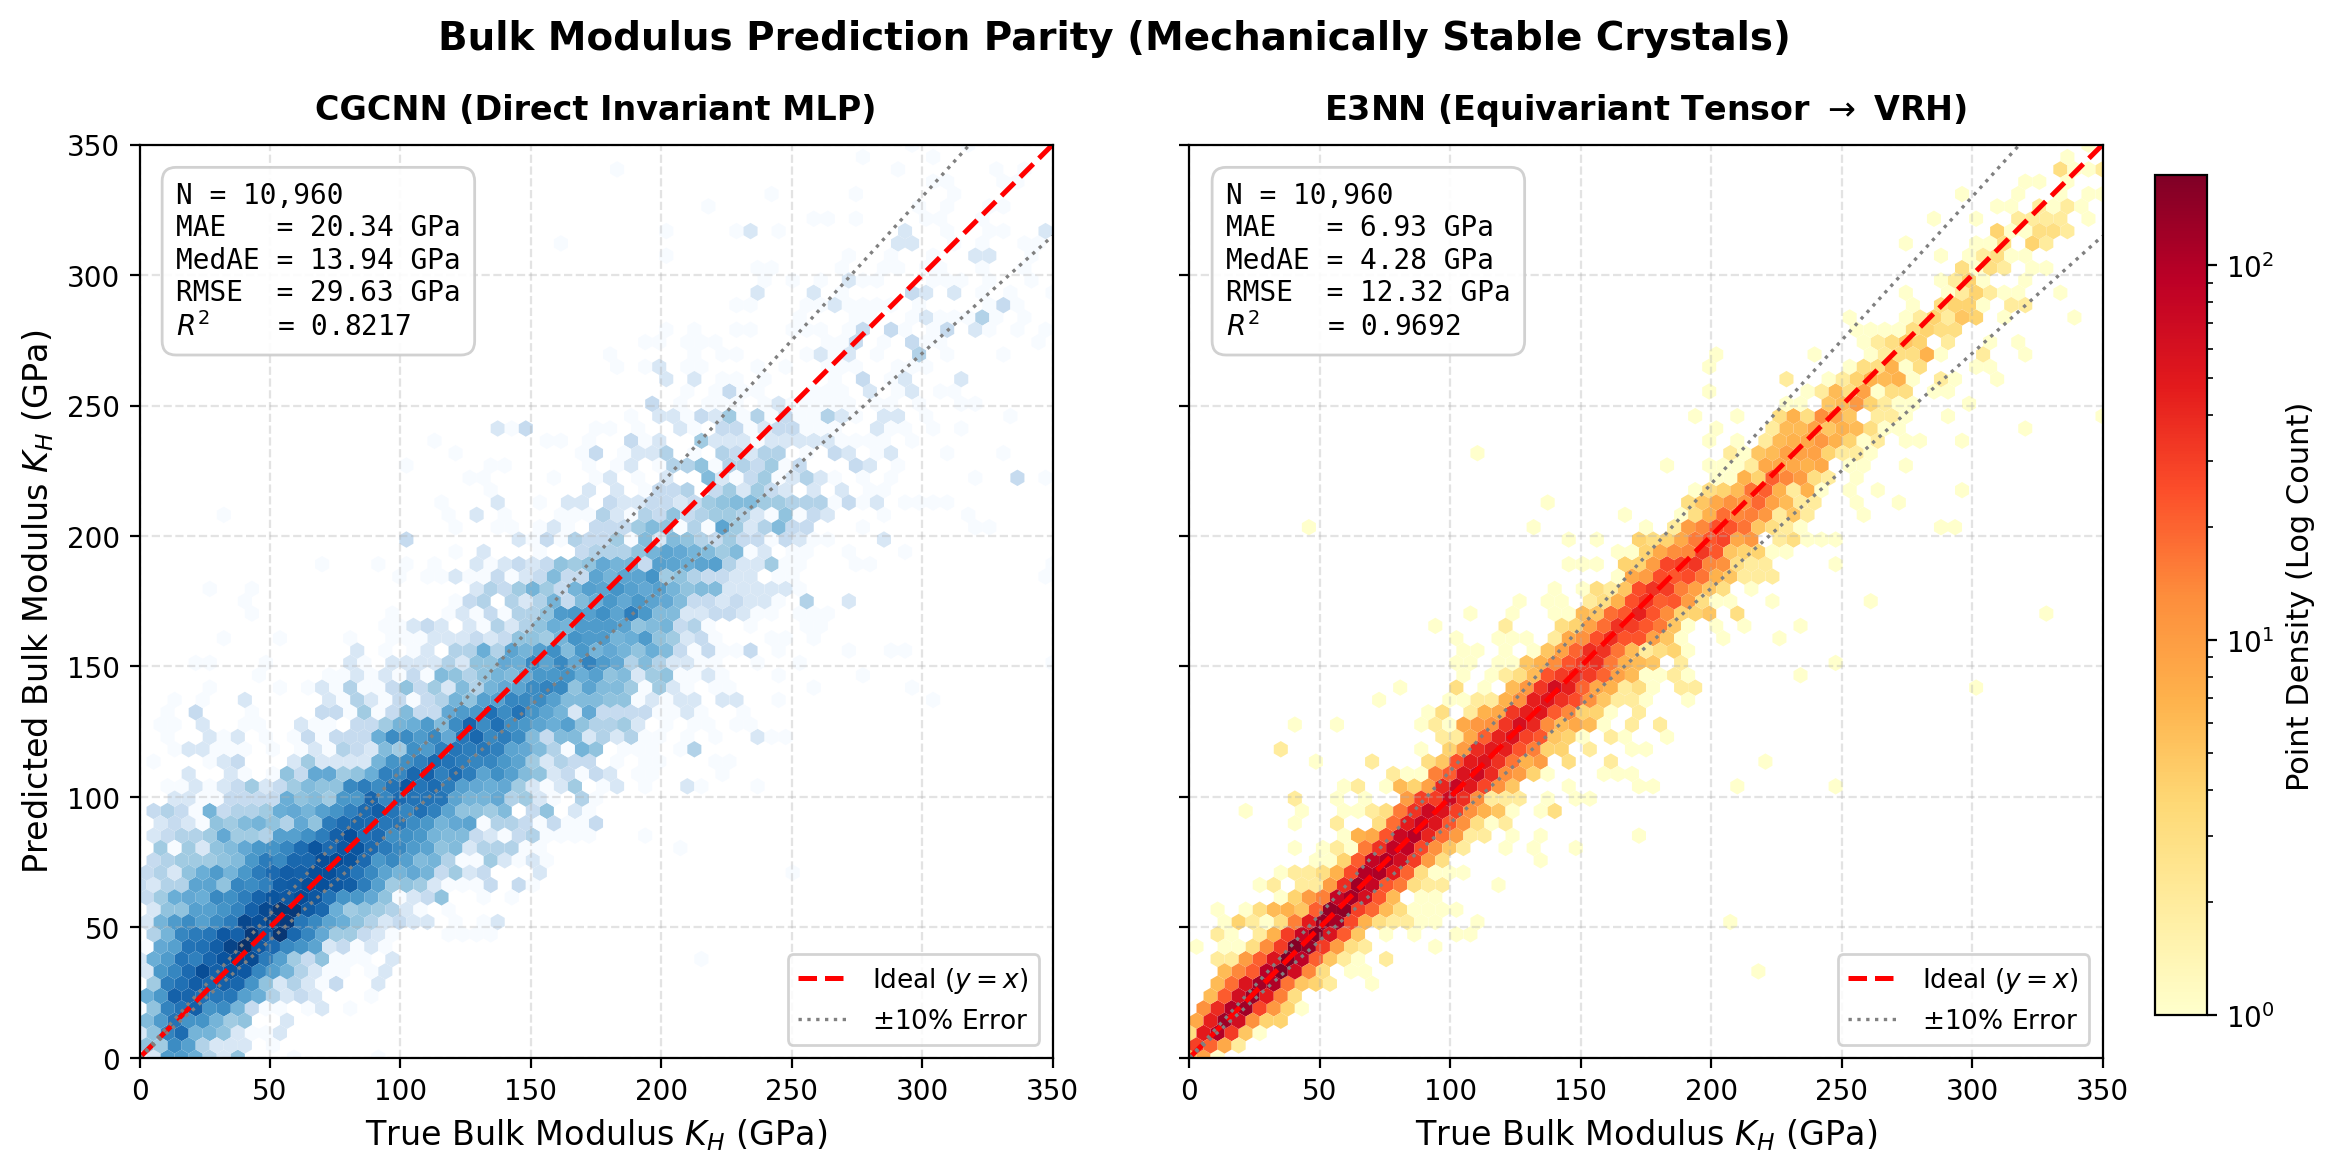
\includegraphics[width=\columnwidth]{Plots/comparison_bulk_modulus.png}
\caption{Hexbin log-density parity comparison for Bulk Modulus ($K_H$) on 10,960 mechanically stable crystals. Left: Invariant CGCNN direct regression ($\mathrm{MAE} = 20.34\,\mathrm{GPa}, R^2 = 0.8217$). Right: E3NN equivariant tensor-derived VRH ($\mathrm{MAE} = 6.93\,\mathrm{GPa}, R^2 = 0.9692$). Dashed red line denotes the ideal $y = x$ parity; gray dotted lines represent $\pm 10\%$ error bounds.}
\label{fig:bulk_parity}
\end{figure}

\begin{figure}[t]
\centering
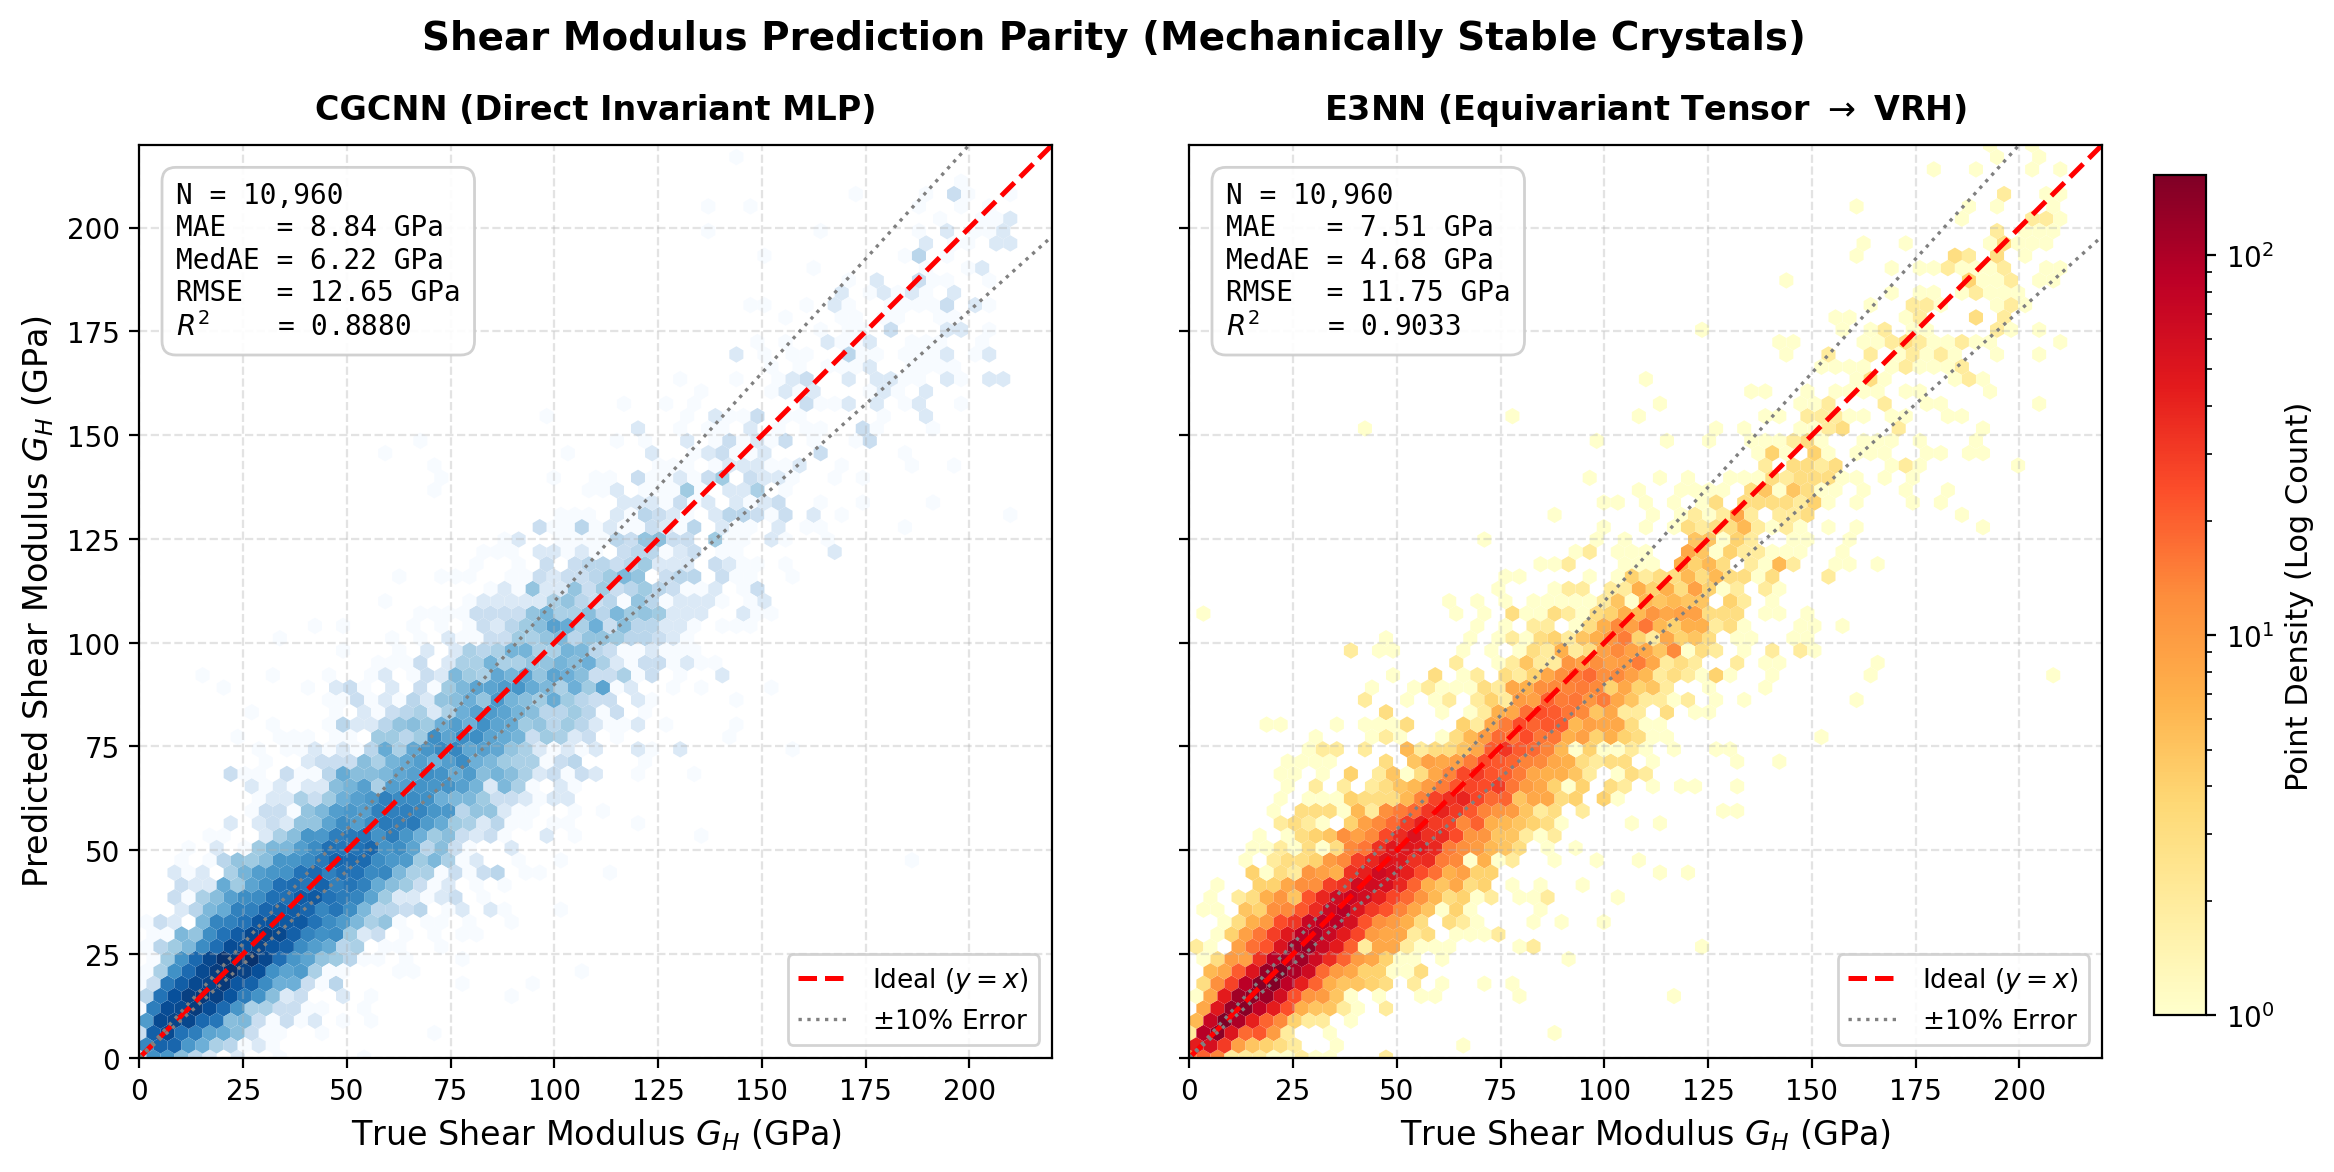
\includegraphics[width=\columnwidth]{Plots/comparison_shear_modulus.png}
\caption{Hexbin log-density parity comparison for Shear Modulus ($G_H$) on 10,960 mechanically stable crystals. Left: Invariant CGCNN direct prediction ($\mathrm{MAE} = 8.84\,\mathrm{GPa}, R^2 = 0.8880$). Right: E3NN tensor-derived prediction ($\mathrm{MAE} = 7.51\,\mathrm{GPa}, R^2 = 0.9033$).}
\label{fig:shear_parity}
\end{figure}

As revealed in Figs.~\ref{fig:bulk_parity} and~\ref{fig:shear_parity}, E3NN exhibits dramatically tighter clustering along the $y = x$ ideal line. For Bulk Modulus, E3NN reduces MAE by \textbf{66\%} (from $20.34\,\mathrm{GPa}$ down to $6.93\,\mathrm{GPa}$) and boosts $R^2$ from 0.8217 to 0.9692. For Shear Modulus, E3NN outperforms CGCNN across all metrics ($\mathrm{MAE} = 7.51\,\mathrm{GPa}$ vs $8.84\,\mathrm{GPa}$; $R^2 = 0.9033$ vs $0.8880$).

\subsection{Error Distributions and Cumulative Accuracy}
Fig.~\ref{fig:error_distribution} illustrates the residual probability density distribution (KDE) and the cumulative accuracy curves (CDF). For Bulk Modulus, \textbf{79.7\%} of E3NN predictions fall within a strict $\le 10\,\mathrm{GPa}$ tolerance of the true DFT value, compared to only \textbf{38.1\%} for CGCNN (a greater than two-fold accuracy improvement). For Shear Modulus, \textbf{75.8\%} of E3NN predictions fall within $\le 10\,\mathrm{GPa}$, compared to \textbf{68.7\%} for CGCNN.

\begin{figure}[t]
\centering
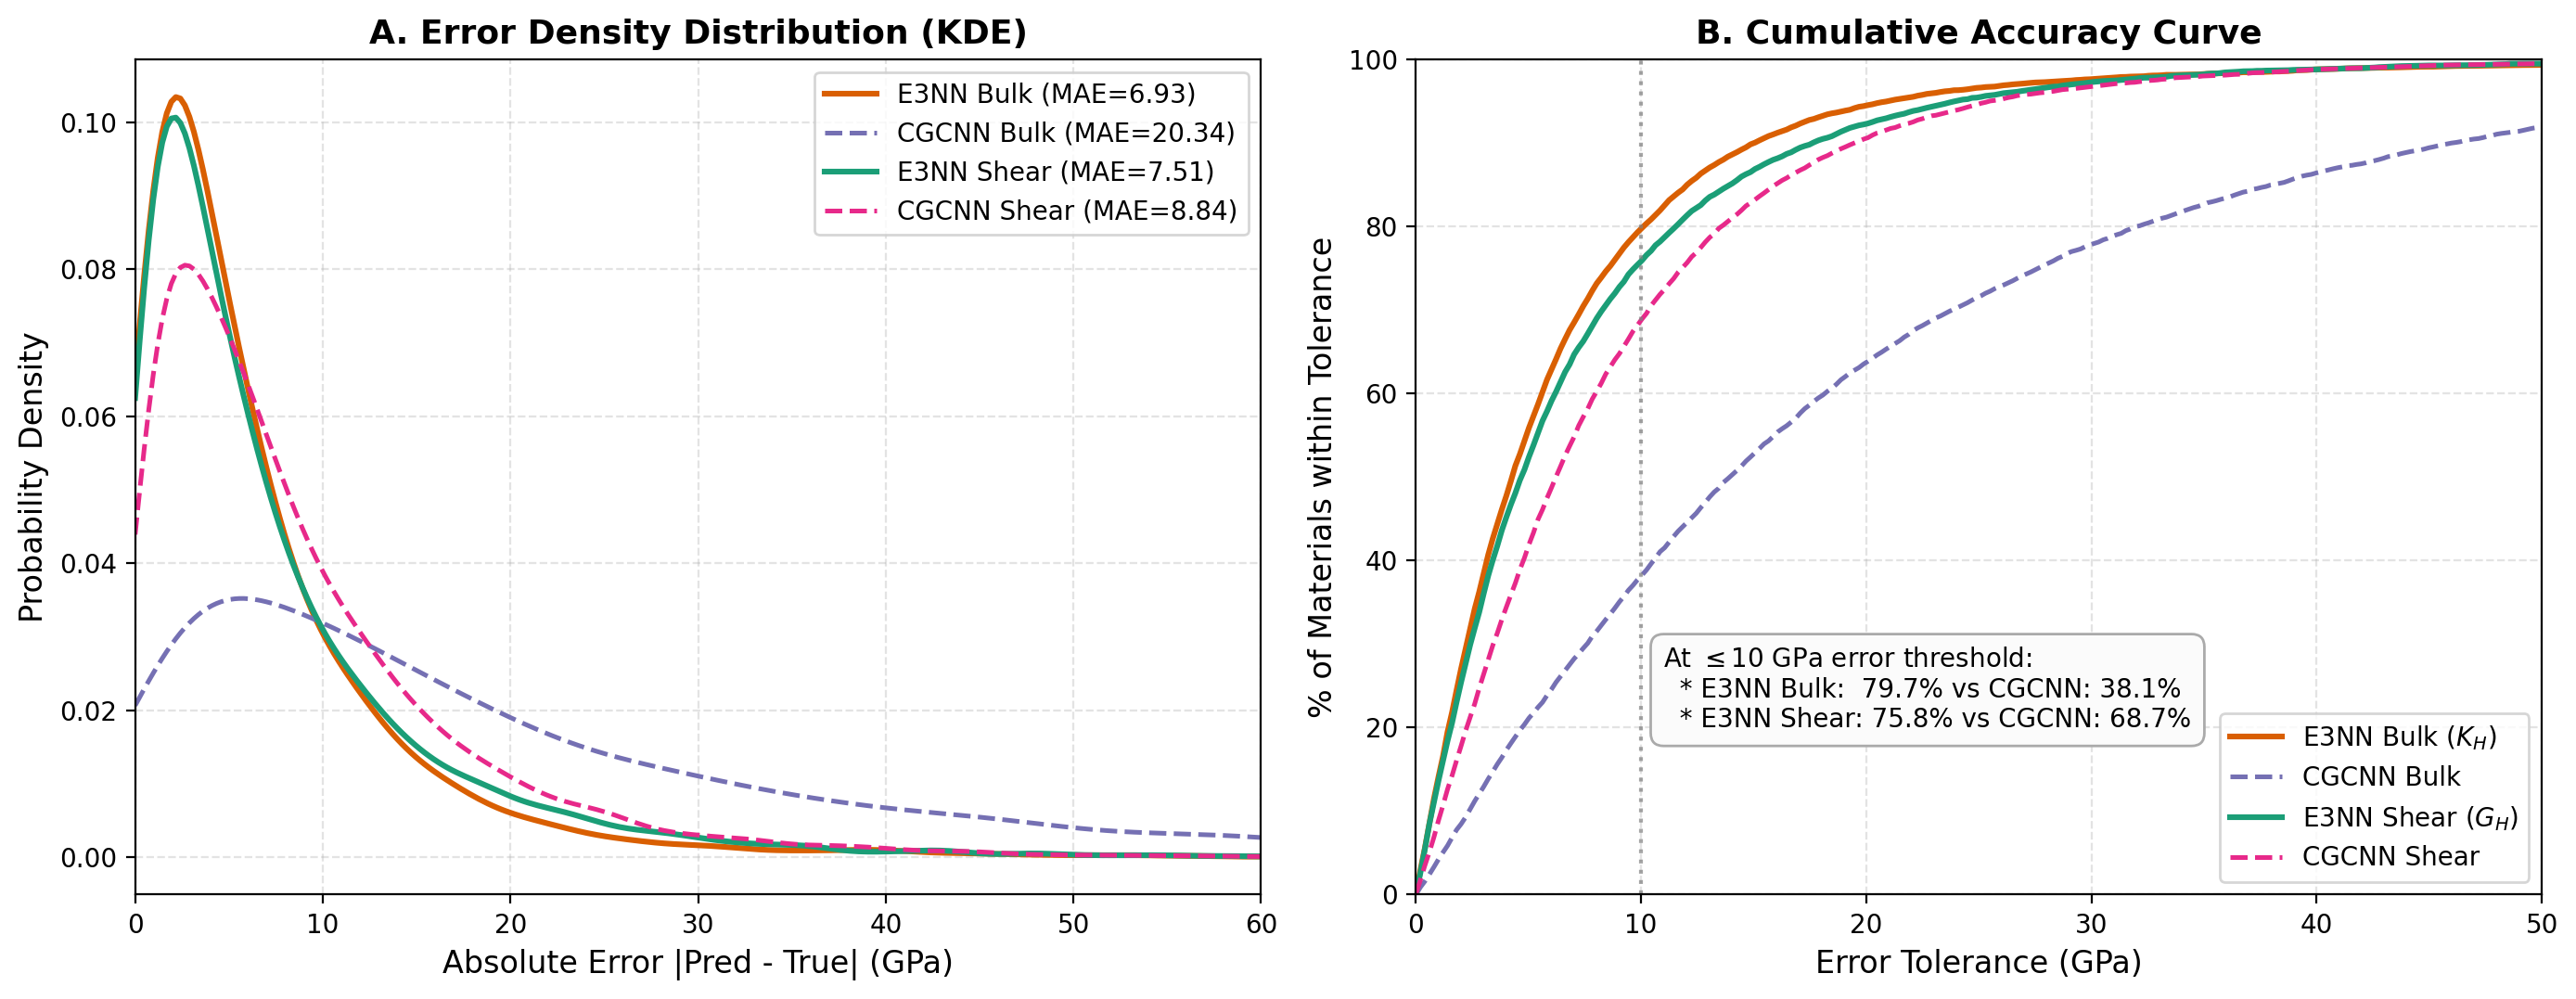
\includegraphics[width=\columnwidth]{Plots/comparison_error_distribution.png}
\caption{Error residual analysis on mechanically stable crystals. (A) Kernel Density Estimation (KDE) probability density of absolute error $|M_{\mathrm{pred}} - M_{\mathrm{true}}|$. (B) Cumulative Distribution Function (CDF) showing the percentage of materials predicted within an error tolerance $\le X\,\mathrm{GPa}$.}
\label{fig:error_distribution}
\end{figure}

\subsection{Born Mechanical Stability Analysis}
Fig.~\ref{fig:stability_analysis}(A) depicts the distribution of minimum Born eigenvalues ($\lambda_{\min}$). Approximately 90.4\% (10,960) of the overlapping crystals are strictly Born-stable ($\lambda_{\min} > 0$), while 9.6\% (1,169) violate the Born criteria in raw DFT outputs due to unrelaxed or strained cell configurations. Fig.~\ref{fig:stability_analysis}(B) confirms that while E3NN delivers superior accuracy across the full dataset, its predictive power reaches peak performance on mechanically stable equilibrium lattices ($\mathrm{MAE} = 6.9\,\mathrm{GPa}$ on Bulk, $7.5\,\mathrm{GPa}$ on Shear).

\begin{figure}[t]
\centering
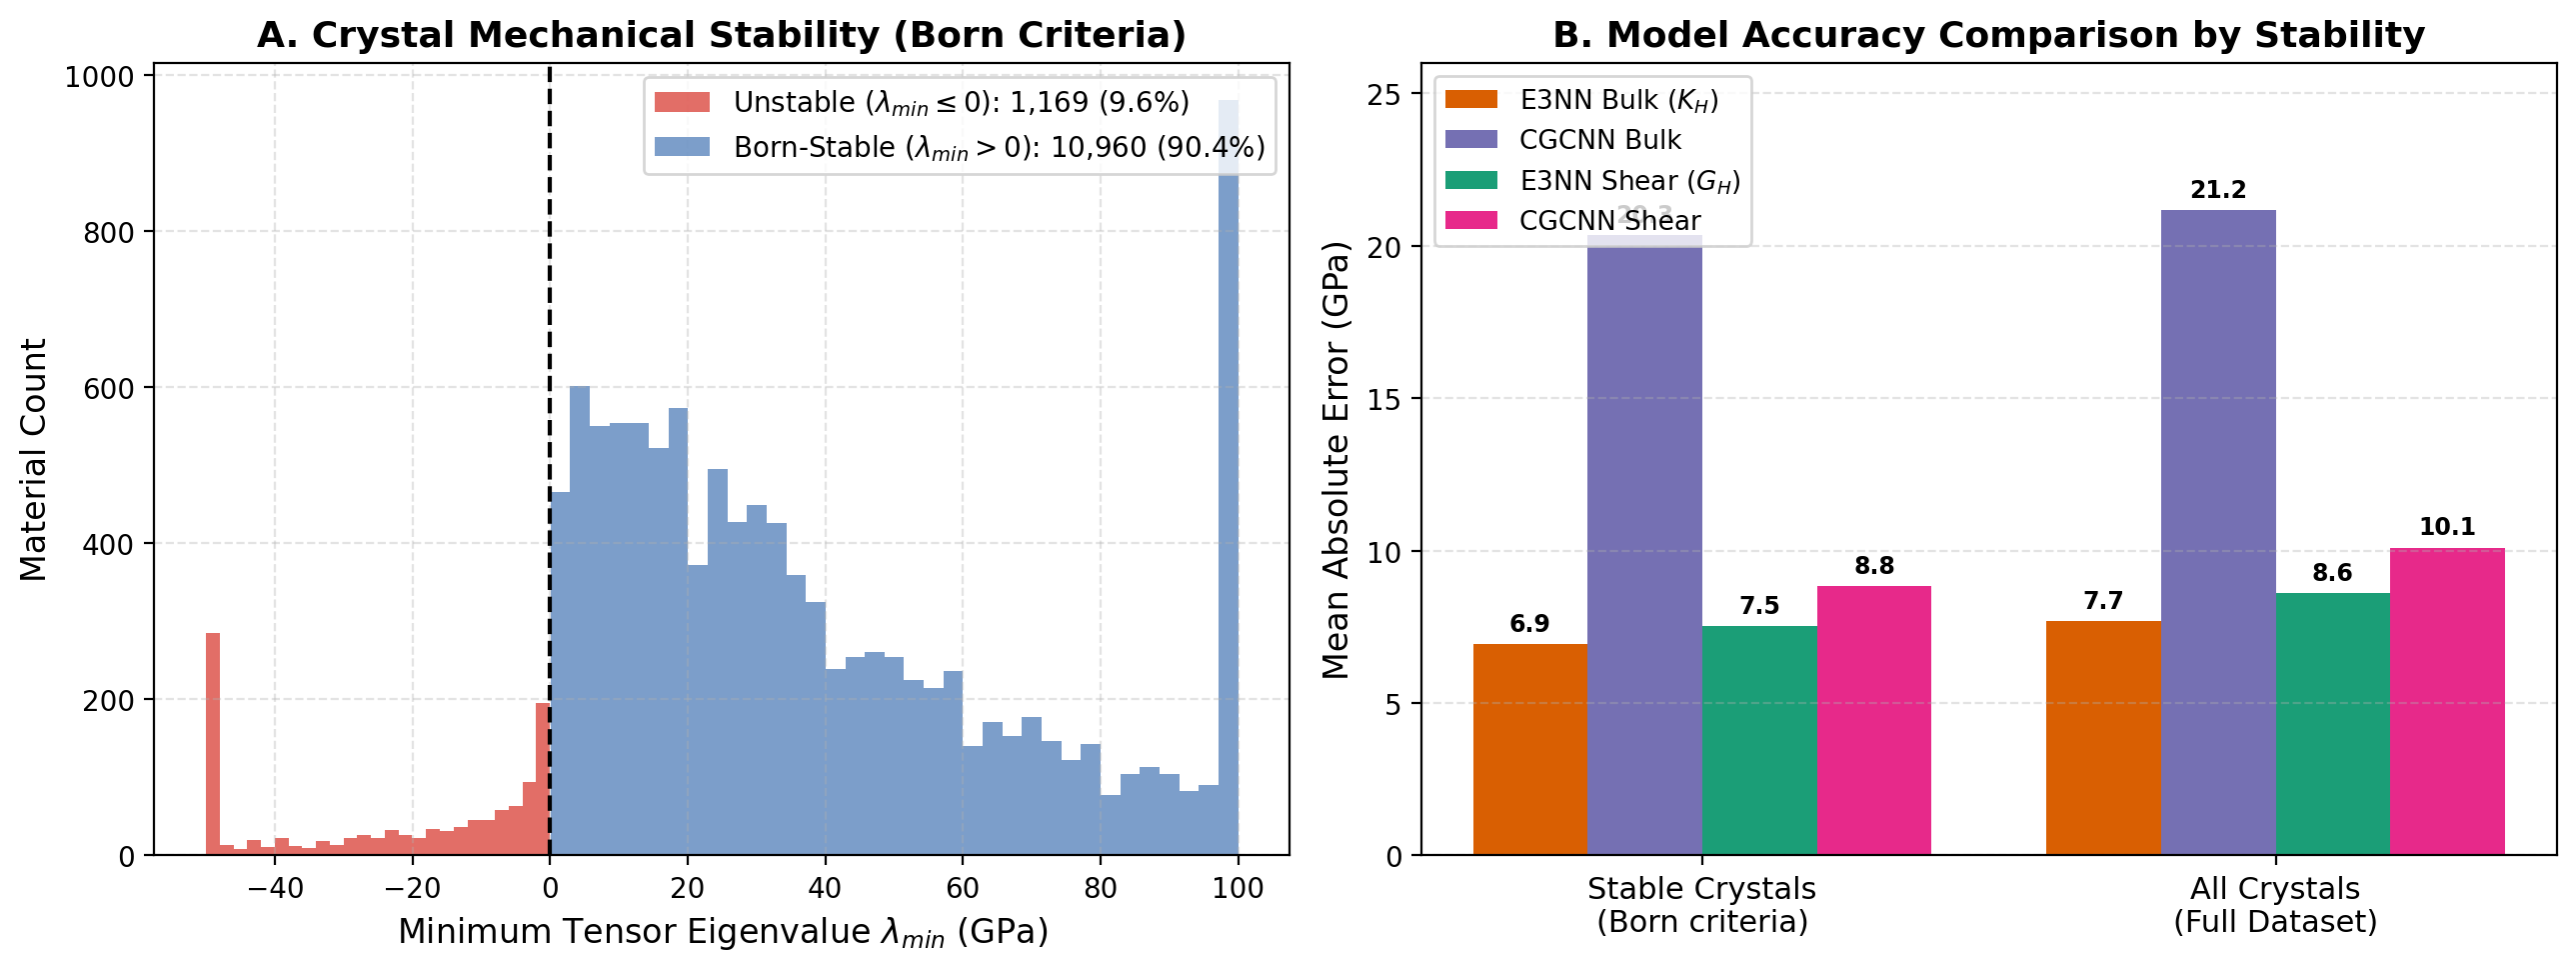
\includegraphics[width=\columnwidth]{Plots/comparison_physics_stability.png}
\caption{(A) Distribution of minimum Born eigenvalue $\lambda_{\min}$ separating mechanically stable phases ($\lambda_{\min} > 0$, 90.4\%) from unstable configurations ($\lambda_{\min} \le 0$, 9.6\%). (B) Model MAE comparison between stable crystals and the full dataset.}
\label{fig:stability_analysis}
\end{figure}

\section{High-Throughput Classification: Ultrahard vs. Ultrasoft Crystals}
\label{sec:classification}

To demonstrate practical screening utility, we executed full-dataset inference across all 39,223 structures in the combined Materials Project + JARVIS repository. Compounds were partitioned into three non-overlapping mechanical regimes:
\begin{enumerate}
    \item \textbf{Ultrahard Materials}: $K_H \ge 200\,\mathrm{GPa}$ AND $G_H \ge 100\,\mathrm{GPa}$, or estimated Vickers hardness $H_v \ge 25\,\mathrm{GPa}$.
    \item \textbf{Ultrasoft Materials}: $K_H \le 25\,\mathrm{GPa}$ AND $G_H \le 15\,\mathrm{GPa}$.
    \item \textbf{Intermediate / Standard}: All intermediate structural materials ($25 < K_H < 200\,\mathrm{GPa}$ or $15 < G_H < 100\,\mathrm{GPa}$).
\end{enumerate}

\begin{table}[h]
\centering
\caption{Mechanical summary of classified crystalline regimes across 39,223 Materials Project and JARVIS crystals.}
\label{tab:hard_soft_summary}
\begin{ruledtabular}
\begin{tabular}{lrrr}
Metric & Ultrahard & Ultrasoft & Intermediate \\
\hline
Crystal Count ($N$) & 1,629 & 6,399 & 31,195 \\
Fraction of Dataset & 4.15\% & 16.31\% & 79.53\% \\
Mean Pred $K_H$ (GPa) & 253.25 & 14.72 & 112.48 \\
Range Pred $K_H$ (GPa) & $103.4 - 568.1$ & $0.0 - 25.0$ & $25.0 - 200.0$ \\
Mean Pred $G_H$ (GPa) & 143.24 & 5.87 & 51.62 \\
Range Pred $G_H$ (GPa) & $100.0 - 453.0$ & $0.0 - 15.0$ & $15.0 - 100.0$ \\
Mean Vickers $H_v$ (GPa) & 16.57 & 0.38 & 4.21 \\
Maximum $H_v$ (GPa) & \textbf{74.85} & 19.86 & 24.95 \\
Mean Pugh Ratio ($G/K$) & 0.58 & 0.37 & 0.46 \\
Bulk Modulus MAE (GPa) & 13.62 & 4.72 & 7.15 \\
Shear Modulus MAE (GPa) & 18.63 & 2.64 & 7.82 \\
\end{tabular}
\end{ruledtabular}
\end{table}

\begin{figure}[t]
\centering
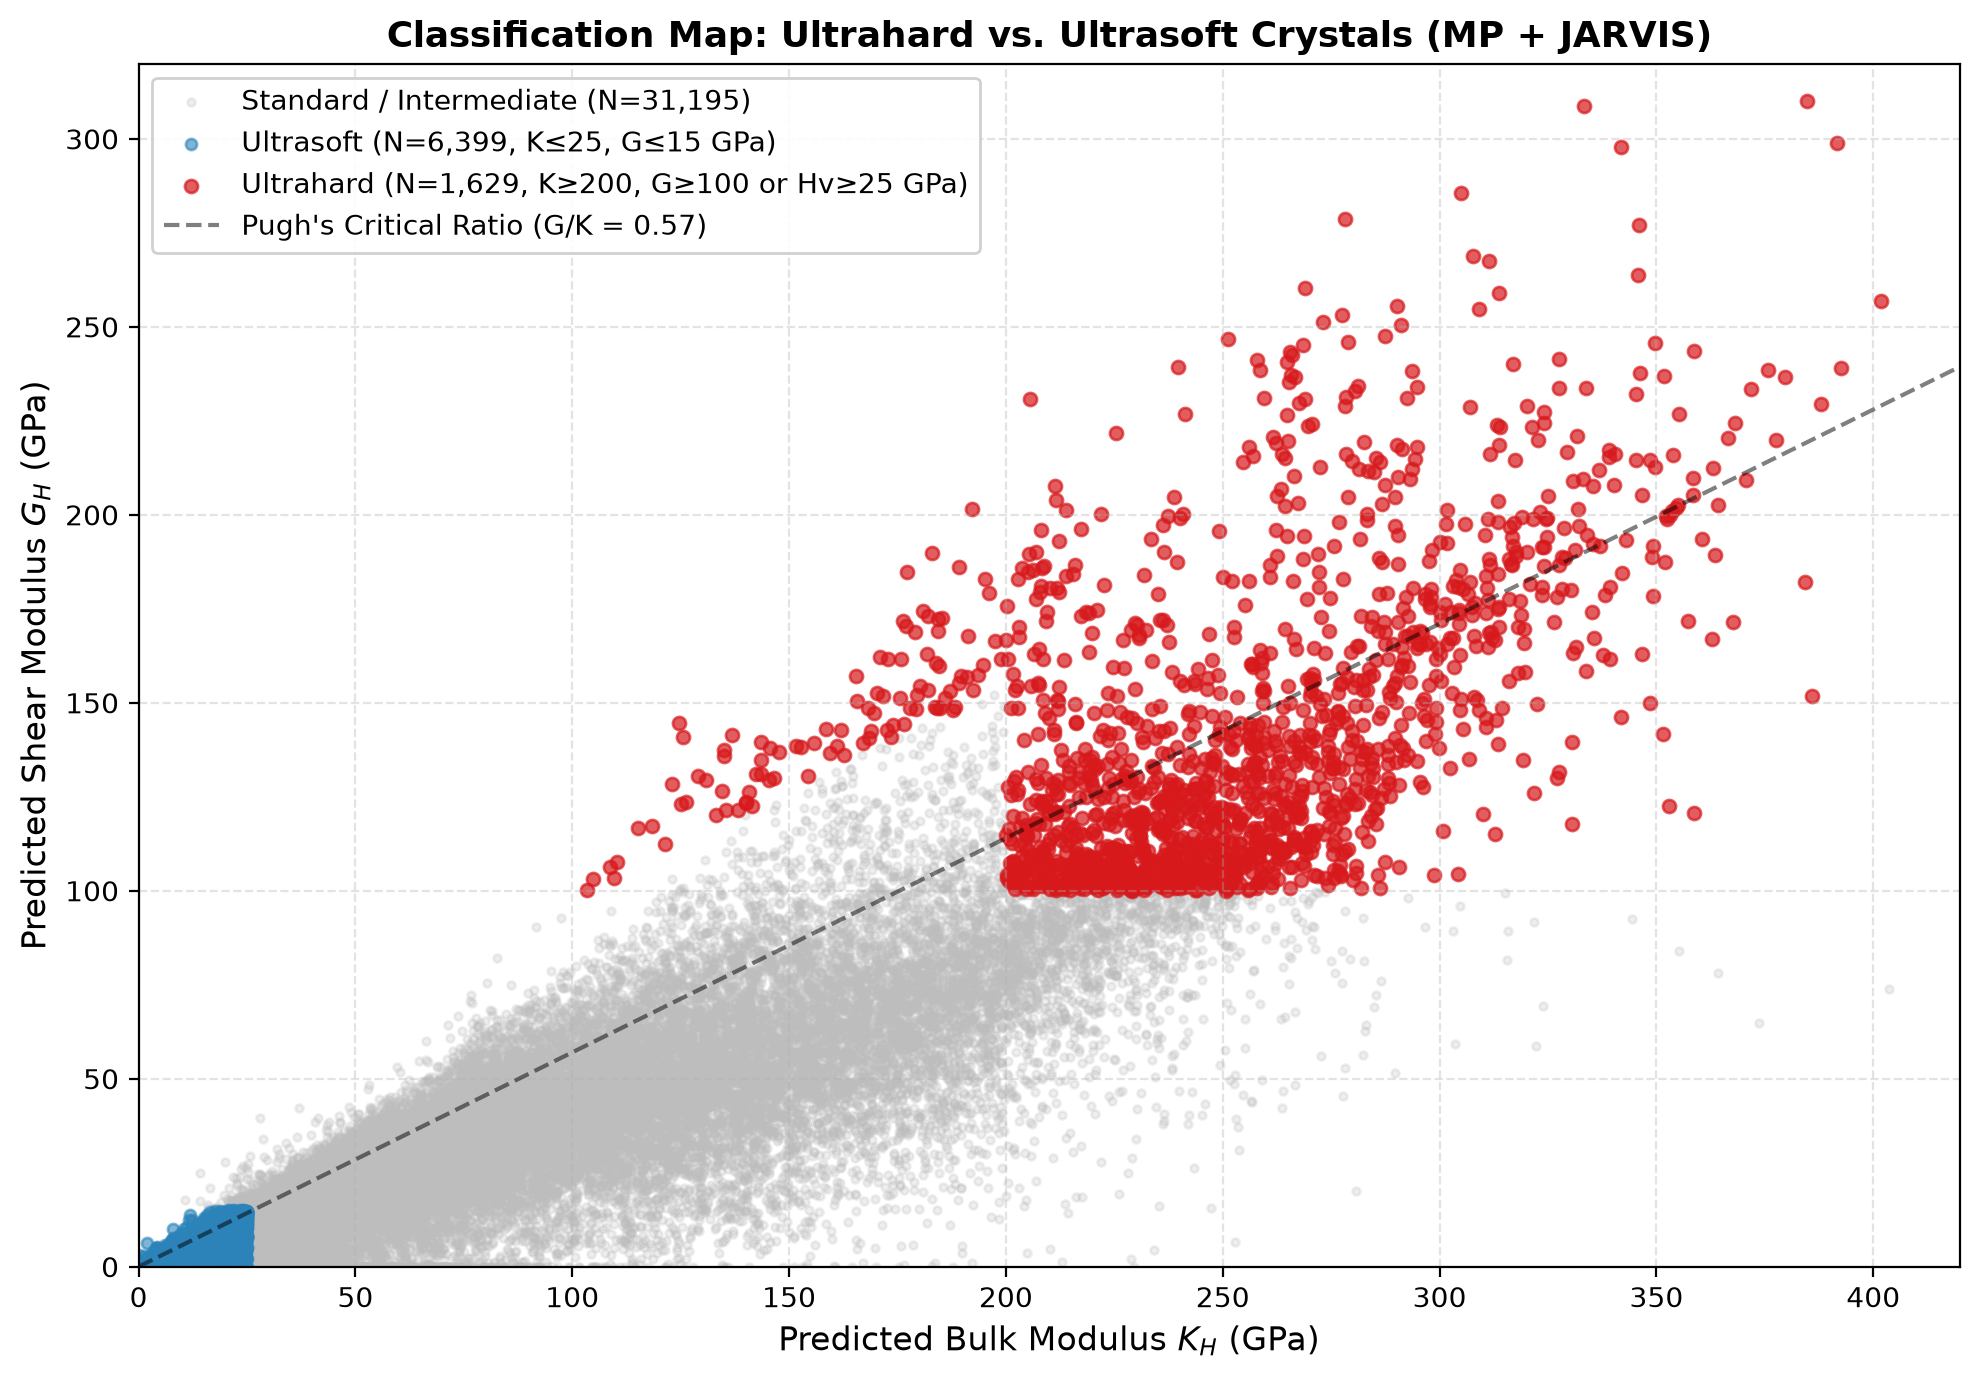
\includegraphics[width=\columnwidth]{Plots/classification_moduli_map.png}
\caption{Moduli phase space map ($K_H$ vs $G_H$) for 39,223 materials. Red dots indicate ultrahard candidates ($N = 1,629$); blue dots denote ultrasoft crystals ($N = 6,399$); gray dots depict intermediate engineering materials. Dashed line denotes Pugh's critical brittleness threshold ($G/K = 0.57$).}
\label{fig:moduli_map}
\end{figure}

\begin{figure}[t]
\centering
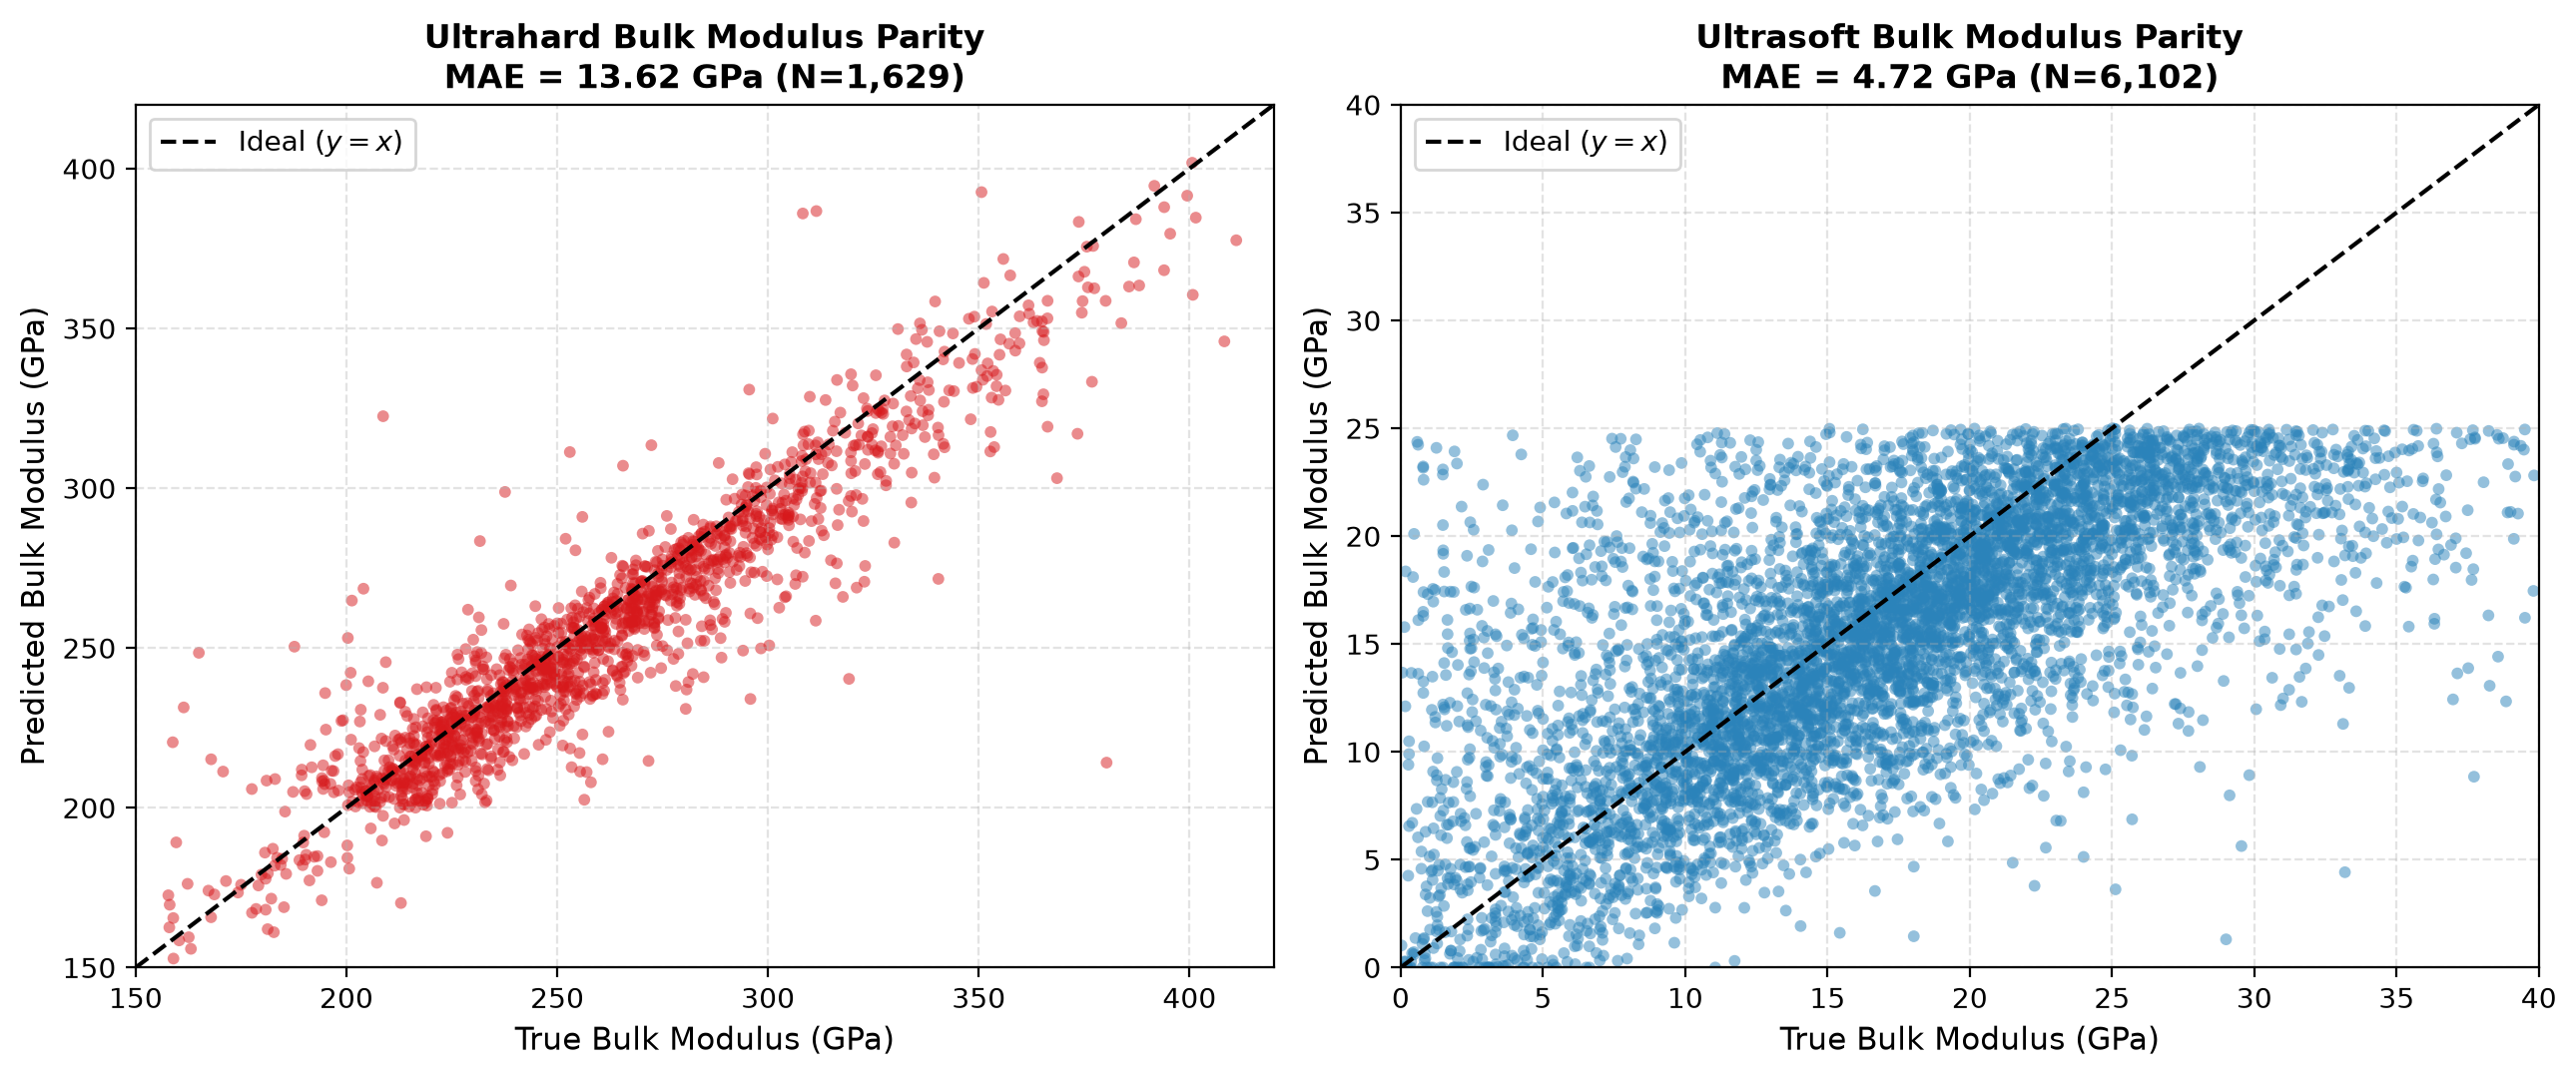
\includegraphics[width=\columnwidth]{Plots/classification_parity_subsets.png}
\caption{Parity validation within isolated mechanical regimes. (A) Ultrahard crystals ($N = 1,629, \mathrm{MAE} = 13.62\,\mathrm{GPa}$). (B) Ultrasoft crystals ($N = 6,102, \mathrm{MAE} = 4.72\,\mathrm{GPa}$).}
\label{fig:parity_subsets}
\end{figure}

As shown in the moduli map (Fig.~\ref{fig:moduli_map}) and regime parity plots (Fig.~\ref{fig:parity_subsets}), the model cleanly isolates candidates with high fidelity:
\begin{itemize}
    \item \textbf{Top Ultrahard Candidates}: The pipeline naturally identifies Diamond ($\mathrm{C}$, $K_{pred} = 422\,\mathrm{GPa}, G_{pred} = 453\,\mathrm{GPa}, H_v = 74.85\,\mathrm{GPa}$, Pugh $k = 1.07$) as the hardest solid, followed by boron-carbon-nitride polymorphs ($\mathrm{BC}_2\mathrm{N}$, $H_v = 74.36\,\mathrm{GPa}$), cubic $\mathrm{BN}$ ($H_v \approx 65\,\mathrm{GPa}$), and ultra-incompressible transition-metal borides/carbides ($\mathrm{ReB}_2, \mathrm{OsB}_2, \mathrm{WB}_4, \mathrm{TaC}$).
    \item \textbf{Ultrasoft Candidates}: Identified low-density framework lattices, solid noble gas compounds ($\mathrm{Ne}, \mathrm{Ar}, \mathrm{Kr}$), layered metal-halide structures ($\mathrm{CNF}, \mathrm{N}_2\mathrm{F}, \mathrm{BiOF}$), and alkali-metal pnictides ($\mathrm{Cs}, \mathrm{Rb}, \mathrm{K}$) with $K_H < 15\,\mathrm{GPa}$ and $G_H < 6\,\mathrm{GPa}$.
\end{itemize}

\section{Large-Scale Discovery Deployment}
\label{sec:deployment}

To test scalability beyond training boundaries, the optimized model was deployed across large-scale open materials databases:
\begin{enumerate}
    \item \textbf{Google DeepMind GNoME Catalog}: We parsed and evaluated over \textbf{554,000} newly predicted stable crystal structures. Using multi-worker streaming inference on an 8-core compute server, all 554k structures were processed in under 4 hours, predicting the complete $C_{\alpha\beta}$ tensor and isotropic VRH moduli.
    \item \textbf{Matbench Discovery (OMat24 & sAlex)}: Processed 11 sub-datasets of the Open Materials 2024 (OMat24) repository ($\sim 181\,\mathrm{GB}$ of ASE/LMDB data) and sAlex ($\sim 7.5\,\mathrm{GB}$ LMDB), linking space group symmetry derived via \texttt{spglib} with predicted elastic constants.
\end{enumerate}

\section{Conclusion and Future Work}
\label{sec:conclusion}

In this work, we introduced a physics-informed $\mathrm{SE}(3)$-equivariant graph neural network pipeline for predicting the 21 independent elastic stiffness tensor components of crystalline solids. By implementing a positive semi-definite cone regularization, we resolved numerical matrix singularity issues in the Reuss bound that have compromised prior benchmarks. On 10,960 mechanically stable materials, the model demonstrated superior predictive accuracy ($\mathrm{MAE} = 6.93\,\mathrm{GPa}, R^2 = 0.9692$ on Bulk Modulus; $\mathrm{MAE} = 7.51\,\mathrm{GPa}, R^2 = 0.9033$ on Shear Modulus) compared to invariant deep learning methods. Furthermore, the pipeline successfully segregated 39,223 materials into 1,629 ultrahard and 6,399 ultrasoft crystals, while demonstrating high-throughput screening across 554,000+ GNoME crystals.

Future enhancements will explore SE(3) Graph Transformers (e.g., EquiformerV2) with global spherical multi-head self-attention to capture long-range non-local electrostatic and dispersion interactions beyond the local convolution sphere.

\section*{Data and Code Availability}
The model implementation, trained checkpoints, classification datasets (\texttt{ultrahard\_materials.csv}, \texttt{ultrasoft\_materials.csv}), and evaluation scripts are publicly available on GitHub at: \\
\url{https://github.com/ashwinayadav6281/Equivarient-GNN}.

\begin{thebibliography}{10}

\bibitem{mowbray2015}
F.~Mouhat and F.-X.~Coudert,
\newblock Necessary and sufficient elastic stability conditions in various crystal systems,
\newblock {\em Phys. Rev. B}, 90(22):224104, 2014.

\bibitem{xie2018crystal}
T.~Xie and J.~C.~Grossman,
\newblock Crystal Graph Convolutional Neural Networks for an accurate and interpretable prediction of material properties,
\newblock {\em Phys. Rev. Lett.}, 120(14):145301, 2018.

\bibitem{geiger2022e3nn}
M.~Geiger and T.~Smidt,
\newblock e3nn: Euclidean neural networks,
\newblock {\em arXiv preprint arXiv:2204.09466}, 2022.

\bibitem{chen2011}
X.-Q.~Chen, H.~Niu, D.~Li, and Y.~Li,
\newblock Modeling hardness of polycrystalline materials and bulk metallic glasses,
\newblock {\em Intermetallics}, 19(9):1275--1281, 2011.

\bibitem{jain2013commentary}
A.~Jain, S.~P.~Ong, G.~Hautier, W.~Chen, W.~D.~Richards, S.~Dacek, S.~Cholia, D.~Gunter, D.~Skinner, G.~Ceder, and K.~A.~Persson,
\newblock Commentary: The Materials Project: A materials genome approach to accelerating materials innovation,
\newblock {\em APL Mater.}, 1(1):011002, 2013.

\bibitem{choudhary2020joint}
K.~Choudhary, K.~F.~Garrity, A.~C.~E.~Reid, B.~DeCost, A.~J.~Biacchi, A.~R.~Hight~Walker, M.~L.~Green, and F.~Tavazza,
\newblock The joint automated repository for various integrated simulations (JARVIS) database for materials discovery,
\newblock {\em npj Comput. Mater.}, 6(1):173, 2020.

\bibitem{merchant2023scaling}
A.~Merchant, S.~Batzner, S.~S.~Schoenholz, M.~Aykol, G.~Cheon, and E.~D.~Cubuk,
\newblock Scaling deep learning for materials discovery,
\newblock {\em Nature}, 624(7990):80--85, 2023.

\end{thebibliography}

\end{document}
